\chapter{A Review of Variational Auto-Encoders}
\label{sec:background}


Given samples from a data distribution $\pdata(\rvx)$, a variational auto-encoder or VAE~\citep{kingma2013auto,rezende2014stochastic} learns an approximation of this data distribution which we can sample from. We denote this distribution $p_\theta(\rvx)$, where $\theta$ denotes learnable parameters of the VAE. The data distribution $\pdata(\rvx)$ can be complex. Since complex distributions are hard to parameterize with a neural network, VAEs introduce the notion of a latent variable $\rvz \in \gZ$ and break the process of generating data into two steps: in the first step they sample a latent variable $\rvz$ from a ``prior'' distribution $p_\theta(\rvz)$. The prior distribution can be fixed, \eg a unit Gaussian, or can have learnable parameters that are included in $\theta$. In the second step, the VAE parameterizes a ``likelihood'' $p_\theta(\rvx|\rvz)$. This can be, \eg, a Gaussian for continuous data~\citep{kingma2013auto} or a categorical for discrete data~\citep{child2020very}, with parameters output in either case by a neural network as a function of $\rvz$. Through these two distributions, the VAE parameterizes a distribution in data-space that can be obtained by marginalizing over the latent variable:
\begin{equation} \label{eq:vae-marginal}
p_\theta(\rvx) = \int p_\theta(\rvx|\rvz)p_\theta(\rvz) \mathrm{d}\rvz.
\end{equation}
Even if both the prior $p_\theta(\rvz)$ and likelihood $p_\theta(\rvx|\rvz)$ are simple distributions, the marginal $p_\theta(\rvx)$ can be complex since the parameters of the likelihood can be arbitrarily complex functions of $\rvz$.

Ideally, the parameters $\theta$ would be learned to
maximise the average of $\log p_\theta(\rvx)$ over all training examples, which corresponds to learning parameters which maximise the likelihood of the dataset under the learned distribution. The required marginalisation in \cref{eq:vae-marginal}, however, is typically intractable. An workaround is to use a proposal distribution $q(\rvz)$ to obtain a lower-bound of the log-marginal. Starting by taking the log of both sides of \cref{eq:vae-marginal}, we see that our objective can be converted to the log of an expectation over $q(\rvz)$:
\begin{align}
\log p_\theta(\rvx) &= \log \int p_\theta(\rvx|\rvz)p_\theta(\rvz) \mathrm{d}\rvz \\
    &= \log \int p_\theta(\rvx|\rvz) \frac{p_\theta(\rvz)}{q(\rvz)} q(\rvz) \mathrm{d}\rvz \\
    &= \log \EX_{q(\rvz)} \left[ p_\theta(\rvx|\rvz) \frac{p_\theta(\rvz)}{q(\rvz)} \right]. \label{eq:vae-marginal-is}
\end{align}
Ideally we would be able to obtain an unbiased estimate of this objective. Due to the order of the expectation and logarithm operators this is not feasible but, using Jensen's inequality, we can obtain a lower bound by switching their order: 
\begin{align}
    \log p_\theta(\rvx) &\geq \EX_{q(\rvz)} \left[ \log p_\theta(\rvx|\rvz) + \log \frac{p_\theta(\rvz)}{q(\rvz)} \right].
    % &= \EX_{q(\rvz)} \left[ \log p_\theta(\rvx|\rvz) \right] + \kl{q(\rvz)}{p_\theta(\rvz)}
\label{eq:marginal-is}
\end{align}
This lower-bound can be stochastically estimated by sampling $\rvz$ from $q(\rvz)$ and evaluating the terms inside the expectation with that given $\rvz$. The tightness of this lower-bound is strongly dependent on how ``good'' the proposal distribution $q(\rvz)$ is. Additionally, the optimal proposal for estimating this bound depends on $\rvx$ so the same proposal cannot necesssarily be used to estimate this bound for different training examples. Therefore \citet{kingma2013auto} propose to train an ``encoder'' with parameters $\phi$ which maps from training examples $\rvx$ to the parameters of the corresponding proposal distributions $q_\phi(\rvz|\rvx)$. This leads to the lower-bound
\begin{align} \label{eq:vae-objective}
    \log p_\theta(\rvx) &\geq \EX_{q_\phi(\rvz|\rvx)} \left[ \log p_\theta(\rvx|\rvz) + \log \frac{p_\theta(\rvz)}{q_\phi(\rvz|\rvx)} \right] = \gL(\rvx, \theta, \phi).
\end{align}
A key insight is that both the encoder parameters $\phi$ and the prior/decoder parameters $\theta$ can be trained to maximize this lower-bound since, if either of them are suboptimal, the bound will decrease. The full optimization problem is therefore to find
\begin{align}
    \argmin_{\theta,\phi} \EX_{\pdata(\rvx)} \left[ \gL(\rvx, \theta, \phi) \right].
\end{align}

\section{Conditional Variational Auto-Encoders}
Our focus in this thesis is on conditional, rather than unconditional, generative models. In the setting we consider we want to approximate the conditional distribution $p_\theta(\rvx|\rvy)$ and at training time have access to either a joint distribution $p_\theta(\rvx,\rvy)$ or a dataset of $(\rvx, \rvy)$ pairs that we can use to approximate the joint distribution.

In order to match the distribution modeled by a VAE to such a conditional distribution, at least one of the prior or decoder should be made conditional on $\rvz$. To cover all cases, we will write both as conditional on $\rvy$. That is, we will denote the prior distribution of a conditional VAE $p_\theta(\rvz|\rvy)$ and the decoder's distribution as $p_\theta(\rvx|\rvy,\rvz)$. The encoder may in principle also be made conditional on $\rvy$, but that is not the case for any of the generative models considered in this thesis and so we will continue to write it as $q_\phi(\rvz|\rvx)$. See \cref{tab:vae_components} for a summary of these differences. The distribution modelled is, as before, obtained by marginalising over $\rvz$ as
\begin{equation} \label{eq:vae-marginal}
p_\theta(\rvx|\rvy) = \int p_\theta(\rvx|\rvy,\rvz)p_\theta(\rvz|\rvy) \mathrm{d}\rvz
\end{equation}
and the training objective for both $\theta$ and $\phi$ is
\begin{equation}
    \gL(\rvx, \rvy, \theta, \phi) = \EX_{q_\phi(\rvz|\rvx)} \left[ \log p_\theta(\rvx|\rvy,\rvz) + \log \frac{p_\theta(\rvz|\rvy)}{q_\phi(\rvz|\rvx)} \right].
\end{equation}

To understand the properties of VAEs, we now take a look at a few ways to decompose this training objective. One is to separate the objective into a reconstruction loss and a KL divergence:
\begin{align}
    \gL(\rvx, \rvy, \theta, \phi) &= \underbrace{\EX_{q_\theta(\rvz|\rvx)} \left[ \log p_\theta(\rvx|\rvz) \right]}_\text{reconstruction loss} + \underbrace{\kl{q_\phi(\rvz|\rvx)}{p_\theta(\rvz)}}_\text{KL divergence},
\label{eq:marginal-is}
\end{align}
The reconstruction loss encourages the encoder and decoder to be learned such that little information is lost if we map a data point $\rvx$ to latent space and back. The KL divergence penalises differences between the encoder's proposal distribution and the prior distribution.

If we consider the expectation of the objective over the data distribution, we can get furhter insight by separating terms into the entropy of the target distribution and a KL divergence:
\begin{align}
  \EX_{\pdata(\rvx,\rvy)} &\left[ \mathcal{L}(\rvx, \rvy, \theta, \phi) \right] \\
  =& \EX_{\pdata(\rvx,\rvy)} \EX_{q_\phi(\rvz|\rvx)} \left[ \log \pdata(\rvx|\rvy) + \log \frac{p_\theta(\rvx,\rvz|\rvy)}{q_\phi(\rvz|\rvx)\pdata(\rvx|\rvy)} \right]\\
    =& -\mathcal{H}\left[ \pdata(\rvx|\rvy) \right] - \kl[\big] { \pdata(\rvx|\rvy) q_\phi(\rvz|\rvx) }{ p_\theta(\rvx,\rvz|\rvy) }. \label{eq:elbo-kl-joints}
\end{align}
where $p_\theta(\rvx,\rvz|\rvy)$ is the joint distribution defined as $p_\theta(\rvx|\rvy,\rvz)p_\theta(\rvz|\rvy)$ and $\mathcal{H}\left[ \pdata(\rvx|\rvy) \right]$ is the differential entropy of the target distribution. While the differential entropy is not guaranteed to be finite in general, it always will be when $\rvx$ is finite, as is common for pixel values in the image and video domains. Since the KL divergence is always non-negative, our training objective is upper-bounded by the differential entropy. Additionally, the KL-divergence is in the direction which causes mass-covering behaviour~\citep{bishop2006pattern} and so we can expect the learned distribution $p_\theta(\rvx|\rvy)$ to assign probability broadly over the data distribution $\pdata(\rvx|\rvy)$, with any missed modes being heavily penalised.

\begin{table}[t]
\centering
% \begin{tabular}{c|c|c|c}
%  & Prior & Decoder & Encoder \\ 
% \hline
% Unconditional VAE & \( p_\theta(\rvz) \) & \( p_\theta(\rvx|\rvz) \) & \( q_\phi(\rvz|\rvx) \) \\
% Conditional VAE & \( p_\theta(\rvz|\rvy) \) & \( p_\theta(\rvx|\rvy,\rvz) \) & \( q_\phi(\rvz|\rvx) \) \\
% \end{tabular}
\begin{tabular}{l|ll|ll}
 & \multicolumn{2}{c|}{Unconditional} & \multicolumn{2}{c}{Conditional} \\ 
\cline{2-5}
& Notation & Definition & Notation & Definition \\ 
\hline
Prior & \( p_\theta(\rvz) \) & primitive  & \( p_\theta(\rvz|\rvy) \) & primitive  \\
Decoder & \( p_\theta(\rvx|\rvz) \) & primitive  & \( p_\theta(\rvx|\rvy,\rvz) \) & primitive \\
Encoder & \( q_\phi(\rvz|\rvx) \) & primitive  & \( q_\phi(\rvz|\rvx) \) & primitive \\
Predictive & \( p_\theta(\rvx) \) & \( \int p_\theta(\rvx|\rvz)p_\theta(\rvz) \mathrm{d}\rvz \)  & \( p_\theta(\rvx|\rvy) \) & \( \int p_\theta(\rvx|\rvy,\rvz)p_\theta(\rvz) \mathrm{d}\rvz \) \\
\end{tabular}
\caption{Comparison of our notation for distributions relating to an unconditional versus a conditional VAE. The prior, decoder, and encoder distributions are primitives directly parameterised by neural networks. The predictive distribution, which we train to match a target distribution, is defined via a marginalisation.}
\label{tab:vae_components}
\end{table}


% We describe VAEs in terms of three components. \textbf{(\rom{1})} A decoder with
% parameters $\theta\in\Theta$ maps from latent variables $\rvz$ to a distribution
% over data $\rvx$, which we call $\pmodel{}(\rvx | \rvz; \theta)$. \textbf{(\rom{2})}
% There is a prior over latent variables, $\pmodel{}(\rvz;\theta)$. This may have
% learnable parameters, which we consider to be part of $\theta$. Together, the
% prior and decoder define a joint distribution, $\pmodel{}(\rvz, \rvx; \theta)$.
% Finally, \textbf{(\rom{3})} an encoder with parameters $\phi\in\Phi$ maps from
% data to an approximate posterior distribution over latent variables, $q(\rvz|\rvx;
% \phi) \approx \pmodel{}(\rvz|\rvx; \theta)$. For simplicity, the distributions over $\rvz$ output by the prior and encoder are parameterized as diagonal Gaussians. The distribution output by the decoder may be another diagonal Gaussian~\citep{kingma2013auto} or may be more complex to e.g. model discrete $\rvx$~\citep{child2020very}.

% Ideally, $\theta$ would be learned to
% maximise the log likelihood $\log\pmodel{}(\rvx; \theta) = \log \int
% \pmodel{}(\rvz, \rvx; \theta) \mathrm{d}\rvz$, averaged over training examples.  Doing so, however, would require a marginalisation over $\rvz$ and so is not tractable. Instead, $\theta$ and $\phi$ are instead trained jointly to maximise
% an average of the evidence lower-bound (ELBO) over each training example $\rvx
% \sim \pdata{}(\cdot)$:
% \begin{align}
%   & \EX_{\pdata{}(\rvx)} \left[ \text{ELBO}(\theta, \phi, \rvx) \right] \\
%   =& \EX_{\pdata(\rvx)} \EX_{q(\rvz|\rvx; \phi)} \left[ \log\frac{\pmodel{}(\rvz; \theta)\pmodel{}(\rvx|\rvz; \theta)}{q(\rvz|\rvx; \phi)} \right] \label{eq:eelbo}\\
%   =& -\mathcal{H}\left[ \pdata(\I) \right] - \kl[\big] { \pdata{}(\rvx)q(\rvz|\rvx; \phi) }{ \pmodel{}(\rvz, \rvx; \theta) }. \label{eq:elbo-kl-joints}
% \end{align}
% The data distribution's entropy, $\mathcal{H}\left[ \pdata(\I) \right]$, is guaranteed to be a finite constant if
% $\rvx$ is discrete (e.g. an image with discrete pixel values), as well as for many continuous distributions. In such cases, maximising the above objective
% will drive $\pmodel{}(\rvz, \rvx; \theta)$ towards
% $\pdata{}(\rvx)q(\rvz|\rvx; \phi)$, and so the marginal $\pmodel{}(\rvx; \theta)$
% towards $\pdata{}(\rvx)$. The KL divergence shown leads to mass-covering
% behaviour from $\pmodel{}(\rvz, \rvx; \theta)$~\citep{bishop2006pattern} so
% $\pmodel{}(\rvx; \theta)$ should assign probability broadly over the data
% distribution $\pdata{}(\rvx)$.

\section{Hierarchical Variational Auto-Encoders} \label{sec:hierarchical-vae}
In this section we introduce the conditional version of a hierarchical VAE, but note that our description can be transferred to the unconditional setting by removing any dependencies on $\rvy$ or setting $\rvy$ to null. A (conditional) hierarchical VAE~\citep{gregor2015draw,kingma2016improving,sonderby2016ladder,klushyn2019learning} is a (conditional) VAE in which the latent variables $\rvz$ have a particular structure. In particular, $\rvz$ is partitioned into $L$ disjoint groups, $\rvz_1,\ldots,\rvz_L$. The prior $p_\theta(\rvz|\rvy) = p_\theta(\rvz_1,\ldots,\rvz_L|\rvy)$ and encoder $q(\rvz|\rvx,\rvy) = q_\phi(\rvz_1,\ldots,\rvz_L|\rvx,\rvy)$ are then factorised to enable them to represent structured distributions over $\rvz$. How these distributions are factorised is a design choice.
The hierarchical VAEs that we will consider in this thesis are ``top-down'' meaning that they factorise the prior and the encoder distributions in the same order~\citep{vahdat2020nvae,child2020very}:
\begin{equation}
    p_\theta(\rvz) = \prod_{l=1}^L p_\theta(\rvz_l|\rvx,\rvz_{<l}) \quad \text{and} \quad q_\phi(\rvz|\rvx) = \prod_{l=1}^L q_\phi(\rvz_l|\rvx,\rvz_{<l})
\end{equation}
where $\rvz_{<l}$ is the set of all latent variable groups from $\rvz_1$ (inclusive) to $\rvz_{l}$ (exclusive) if $l > 1$ and is null otherwise. We show this dependency structure graphically in \cref{fig:vae-vs-hierarchical-vae}.

\begin{figure}
    \centering
    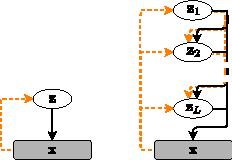
\includegraphics[width=0.5\textwidth]{figs/vae-vs-hierarchical-vae.pdf}
    \caption{A comparison of the dependency structure of a ``standard'' VAE (left) with that of a top-down hierarchical VAE (right). For each, we show the dependencies of each variable in the encoder's distribution though dashed orange lines and the dependencies of each variable in the prior and decoder's distributions with solid black lines. Note that, in the case of a conditional VAE, there are additional dependencies of all prior and decoder distributions on $\rvy$, which we do not show.}
    \label{fig:vae-vs-hierarchical-vae}
\end{figure}

% A hierarchical
% VAEs~\citep{gregor2015draw,kingma2016improving,sonderby2016ladder,klushyn2019learning} can be understood as a VAE in which the latent variables $\rvz$ are partitioned in a way which has been found to improve the
% fidelity of the learned $\pmodel{}(\I{})$, especially for the image
% domain~\citep{vahdat2020nvae,child2020very}. In particular, they define $\rvz$ to
% consist of $L$ disjoint groups, $\rvz_1,\ldots,\rvz_L$. The prior for each $\rvz_l$ can
% depend on the previous groups through the factorisation
% \begin{equation}
%   \label{eq:hierarchical-prior}
%   \pmodel{}(\z{}) = \prod_{l=1}^L \pmodel{}(\z{}_l|\z{}_{<l}).
% \end{equation}
% where $\z{}_{<l}$ is the null set for $l=1$ and $\{\z{}_1,\ldots,\z{}_{l-1}\}$
% otherwise. The distribution
% produced by the encoder for each $\z{}_l$ also depends on the previous hidden
% state $h_{l-1}$ and so factorises as
% $q(\z{}|\I{}) = \prod_{l=1}^L q(\z{}_l|\z{}_{<l}, \I{})$. The distributions
% $\pmodel{}(\z{}_l|\z{}_{<l})$ and $q(\z{}_l|\z{}_{<l}, \I{})$ are commonly parameterized simply as diagonal
% Gaussian distributions~\citep{sonderby2016ladder,vahdat2020nvae,child2020very}.

% \section{Conditional Hierarchical Variational Auto-Encoders}
% There are various ways in which a VAE, or hierarchical VAE, can be modified to become ``conditional'' on information given at test-time~\citet{sohn2015learning,ivanov2018variational}. From now on we will call such information $\rvy$, and assume it is distributed jointly with $\rvx$ in a data distribution $\pdata(\rvx, \rvy)$. The conditional hierarchical VAEs in this thesis work by simply feeding $\rvy$ as an extra input into both the prior and decoder. That is, the decoder will become $\pmodel(\rvx|\rvz, \rvy; \theta)$ and the prior will become $\pmodel(\rvz|\rvy; \theta) = \prod_l \pmodel(\rvz_l|\rvz_{<l},\rvy)$. Optionally, as we will see in \cref{ch:cigcvae}, we can avoid feeding $\rvy$ into the decoder while retaining good performance. This modification leads to the conditional ELBO:
% \begin{align}
%   & \EX_{\pdata{}(\rvx,\rvy)} \left[ \text{ELBO}(\theta, \phi, \rvx, \rvy) \right] \\
%   =& \EX_{\pdata(\rvx,\rvy)} \EX_{q(\rvz|\rvx, \rvy; \phi)} \left[ \log\frac{\pmodel{}(\rvz|\rvy; \theta)\pmodel{}(\rvx|\rvz, \rvy; \theta)}{q(\rvz|\rvx; \phi)} \right] \label{eq:conditional-eelbo}\\
%   =& \EX_{\pdata(\rvy)} \left[ -\mathcal{H}\left[ \pdata(\rvx|\rvy) \right] - \kl[\big] { \pdata{}(\rvx|\rvy)q(\rvz|\rvx,\rvy; \phi) }{ \pmodel{}(\rvz, \rvx; \theta) } \right] . \label{eq:conditional-elbo-kl-joints}
% \end{align}
% This conditional ELBO lower-bounds the expected entropy of the posterior $\pdata(\rvx|\rvy)$ and, when used to optimize $\theta$ and $\phi$, makes our conditional VAE's learned distribution approximate the same posterior $\pdata(\rvx|\rvy)$.

% \section{Diffusion models}
% % \subsection{Hierarchical VAEs with a fixed encoder}
% \label{sec:dm}
% Diffusion models, or DMs~\citep{sohl2015deep,ho2020denoising,nichol2021improved,song2020score}, are another class of generative model. We will describe the conditional extension~\citep{tashiro2021csdi}, in which the modeled $\rvx$ is conditioned on observations $\rvy$. DMs simulate a diffusion process which transforms $\rvx$ to noise, and generate data by learning the probabilistic inverse of the diffusion process. The diffusion process happens over timesteps $0,\ldots,T$ such that $\rvx_0=\rvx$ is data without noise, $\rvx_1$ has a very small amount of noise added, and so on until $\rvx_T$ is almost independent of $\rvx_0$ and approximates a random sample from a unit Gaussian. In the diffusion process we consider, the distribution over $\rvx_t$ depends only on $\rvx_{t-1}$:
% \begin{equation} \label{eq:q-step}
%     q(\rvx_t | \rvx_{t-1}) = \gN(\rvx_t ; \sqrt{\alpha_t}  \rvx_{t-1} , (1-\alpha_t) \rmI ).
% \end{equation}
% Hyperparameters $\alpha_1,\ldots,\alpha_T$ are chosen to all be close to but slightly less than $1$ so that the amount of noise added at each step is small.
% The combination of this diffusion process and a data distribution $q(\rvx_0,\rvy)$ (recalling that $\rvx_0=\rvx$) defines the joint distribution
% \begin{equation} \label{eq:q-joint}
%     q(\rvx_{0:T}, \rvy) = q(\rvx_0, \rvy) \prod_{t=1}^T q(\rvx_t|\rvx_{t-1}).
% \end{equation}
% Recall that $q(\rvx_0, \rvy)$ is simply new notation for the data distribution $\pdata(\rvx,\rvy)$ and the encoder distribution, this equation is analogous to the product of the data distribution and the encoder's distribution
% $\prod_{l=1}^L \pmodel(\rvz|\rvz_{<l})$ in a hierarchical VAE from \cref{sec:hierarchical-vae}. This leads to one perspective on diffusion models as simply a hierarchical VAE in which the encoder has a simple and non-learnable structure.

% DMs work by ``inverting'' the diffusion process: given values of $\rvx_t$ and $\rvy$ a neural network is used to parameterize $p_\theta(\rvx_{t-1}|\rvx_t, \rvy)$, an approximation of $q(\rvx_{t-1}|\rvx_t,\rvy)$. This neural network lets us draw samples of $\rvx_0$ by first sampling $\rvx_T$ from a unit Gaussian (recall that the diffusion process was chosen so that $q(\rvx_T)$ is well approximated by a unit Gaussian), and then iteratively sampling $\rvx_{t-1} \sim p_\theta(\cdot|\rvx_t,\rvy)$ for $t=T,T-1,\ldots,1$. The joint distribution of sampled $\rvx_{0:T}$ given $\rvy$ is
% \begin{equation} \label{eq:p-joint}
%     p_\theta(\rvx_{0:T}|\rvy) = p(\rvx_{T}) \prod_{t=1}^T p_\theta(\rvx_{t-1}|\rvx_t, \rvy)
% \end{equation}
% where $p(\rvx_{T})$ is a unit Gaussian that does not depend on $\theta$. Training the conditional DM therefore involves fitting $p_\theta(\rvx_{t-1}|\rvx_t,\rvy)$ to approximate $q(\rvx_{t-1}|\rvx_t, \rvy)$ for all choices of $t$, $\rvx_t$, and $\rvy$.

% Several observations have been made in recent years which simplify the learning of $p_\theta(\rvx_{t-1}|\rvx_t,\rvy)$. \citet{sohl2015deep} showed that when $\alpha_t$ is close to 1, $p_\theta(\rvx_{t-1}|\rvx_t)$ is approximately Gaussian~\cite{sohl2015deep}. Furthermore, \citet{ho2020denoising} showed that this Gaussian's variance can be modeled well with a non-learned function of $t$, and that a good estimate of the Gaussian's mean can be obtained from a ``denoising model'' as follows. Given data $\rvx_0$ and unit Gaussian noise $\epsilon$, the denoising model (in the form of a neural network) is fed ``noisy'' data $\rvx_t := \sqrt{\tilde{\alpha}_t} \rvx_0 + \sqrt{1 - \tilde{\alpha}_t} \epsilon$ and trained to recover $\epsilon$ via a mean squared error loss. The parameters $\tilde{\alpha}_t := \prod_{i=1}^t \alpha_i$ are chosen to ensure that the marginal distribution of $\rvx_t$ given $\rvx_0$ is $q(\rvx_t|\rvx_0)$ as derived from \cref{eq:q-step}. Given a weighting function $\lambda(t)$, the denoising loss is
% \begin{equation} \label{eq:dm-loss}
%     \mathcal{L}(\theta) = \E_{q(\rvx_0, \rvy, \epsilon)} \left[ \sum_{t=1}^T \lambda(t) \lVert \epsilon - \epsilon_\theta(\rvx_t, \rvy, t) \rVert_2^2 \right] \quad \text{with} \quad \rvx_t = \sqrt{\tilde{\alpha}_t} \rvx_0 + \sqrt{1 - \tilde{\alpha}_t} \epsilon.
% \end{equation}
% The mean of $p_\theta(\rvx_{t-1}|\rvx_t,\rvy)$ is obtained from the denoising model's output $\epsilon_\theta(\rvx_t, \rvy, t)$ as ${\frac{1}{\alpha_t}\rvx_t - \frac{1-\alpha_t}{\sqrt{1-\tilde{\alpha}_t}}\epsilon_\theta(\rvx_t, \rvy, t)}$.
% If the weighting function $\lambda(t)$ is chosen appropriately, optimising \cref{eq:dm-loss} is equivalent to optimising a lower-bound on the data likelihood under $p_\theta$. In practice, simply setting $\lambda(t) := 1$ for all $t$ can produce more visually compelling results in the image domain~\citep{ho2020denoising}.

% % In our proposed method, as in \citet{tashiro2021csdi}, the shapes of $\rvx_0$ and $\rvy$ sampled from $q(\cdot)$ vary. This is because we want to train a model which can flexibly adapt to e.g. varying numbers of observed frames. To map \cref{eq:dm-loss} to this scenario, note that both $\rvx_0$ and $\rvy$ implicitly contain information about which frames in the video they represent (via the index vectors $\mathcal{X}$ and $\mathcal{Y}$ introduced in the previous section). This information is used inside the neural network $\epsilon_\theta(\rvx_t,\rvy, t)$ so that interactions between frames can be conditioned on the distance between them (as described in the following section) and also to ensure that the sampled noise vector $\epsilon$ has the same shape as $\rvx_0$.

% % \subsection{Continuous-time diffusion}

